\documentclass[12pt]{report}
\usepackage[utf8]{inputenc}
\usepackage[margin=1.2in]{geometry}
\usepackage{graphicx}
\usepackage{float}
\usepackage{subcaption}
\usepackage{amsmath}
\usepackage{amssymb}
\usepackage{ulem}
\usepackage{bm}
\usepackage{framed}
\usepackage{xcolor}
\usepackage{ragged2e}
\usepackage{color}
\usepackage{soul}
\usepackage{cancel}
\graphicspath{ {images/} }
\setlength{\parskip}{1em}
\allowdisplaybreaks


\usepackage{titling}
\newcommand{\subtitle}[1]{%
	\posttitle{%
		\par\end{center}
	\begin{center}\large#1\end{center}
	\vskip0.5em}%
}

\newenvironment{blueframed}[1][blue]
{\def\FrameCommand{\fboxsep=\FrameSep\fcolorbox{#1}{white}}%
\MakeFramed {\advance\hsize-\width \FrameRestore}}
{\endMakeFramed}

\newenvironment{spmatrix}[1]
{\def\mysubscript{#1}\mathop\bgroup\begin{bmatrix}}
{\end{bmatrix}\egroup_{\textstyle\mathstrut\mysubscript}}

\title{Tutorial 12}
\subtitle
{
\textbf{keywords}: exam revision

\textbf{estimated reading time}: 36 minutes
}
\author{Quang Bui}
\date{October 16, 2018}

\begin{document}

\maketitle

\section*{Introduction}
\noindent The \textit{Quotes Information for Asset Risk - September 2018} contains raw data on all quotes created during the month of September for LeasePlan NZ's existing and prospective clients. The status of these quotes is as of 12th of October 2018. Although each quote was created on different days in September, we will assume that this data set was captured in a single time period i.e. a cross-sectional data set. Information about each quote is displayed in the following variables:

\newpage
\section*{Question 2}

\noindent \textcolor{red}{\textbf{This question is based on a question from S1, 2018 final emxa:} A researcher wants to test the Efficient Market Hypothesis (EMH) using weekly percentage returns, denoted by $r_t$, on the New York Stock Exchange composite index. In its strict form the EMH states that information observable to the market prior to week $t$ should not help to predict the return during week $t$. If we use only past information on $r$, the EMH stated as $$E(r_t|r_{t-1}, r_{t-2}, \dots) = E(r_t)$$ One simple way to test that the EMH holds is to specify the following alternative AR(1) model to describe $r_t$: $$r_t = \beta_0 + \beta_1 r_{t-1} + u_t$$ where $E(u_t|r_{t-1}, r_{t-2}, \dots) = 0$ and $Var(u_t|r_{t-1}, r_{t-2}, \dots) = \sigma^2$.}

\noindent \textcolor{red}{Using data from the first week of January 2004 to the third week of April 2018 gives the following estimation: \begin{align*}
		\hat{r}_t &= \underset{(0.096)}{0.086} - \underset{(0.038)}{0.059}r_{t-1} \\
		n &= 689, \quad R^2 = 0.0035, \quad \bar{R}^2 = 0.0020
	\end{align*}}

\noindent \textcolor{red}{(a)}

\noindent \textcolor{red}{i. How would you formulate the null hypothesis that the EMH holds based on (4)? Briefly explain your intuition behind your choice of $H_0$.}

\noindent The EMH states that based returns will not help to explain returns at time $t$ $\therefore$ the null that EMH holds is given by, $$H_0: \beta_1 = 0$$ i.e. weekly percentage returns at time $t-1$ should not help to explain results at time $t$.

\noindent \textcolor{red}{ii. Given the OLS regression results in (5) do you reject or not reject the $H_0$ from i.? Briefly explain.}
\begin{align*}
	H_0&: \beta_1 = 0 \quad (EMH\ does\ hold) \\
	H_1&: \beta_1 \neq 0 \quad (EMH\ does\ not\ hold)
\end{align*} \noindent We are performing a two-sided t-test.
$$t = \dfrac{\hat{\beta}_1 - \beta_1}{se(\hat{\beta}_1)} = \dfrac{\hat{\beta}_1}{se(\hat{\beta}_1)} \sim t_{n-k-1} \quad under\ H_0$$
$$n-k-1 = 689 - 1 - 1 = 687$$
$$t_{calc} = \dfrac{-0.059}{0.038} = 1.553$$
\noindent We perform this two-sided t-test at the 5\% level of significance $\alpha = 0.05$. The critical values can be found from the Stats Table or EViews,
\begin{align*}
	t_{crit} &\approx 1.96 \\
	-t_{crit} &\approx -1.96 
\end{align*}
\noindent For this two-sided t-test, we reject $H_0$ if,
$$t_{calc} > t_{crit}$$ $$OR$$ $$t_{calc} < -t_{crit}$$
\noindent Since $t_{calc} = 1.553 < t_{crit} = 1.96$, we fail to reject the null and conclude that there is insufficient evidence from out sample to suggest that the EMH does not hold.

\noindent \textcolor{red}{(b) The alternative AR(1) model does not preclude that potentially there could be dependence between returns that are more than one week apart.}

\noindent \textcolor{red}{i. If the AR(1) model were the correct specification for describing returns, what type of process would you expect $u_t$ to follow? Provide the properties of this process.}

\noindent If the AR(1) model were the correct specification for describing returns, we would expect the errors in the model to be serially uncorrelated, $$cov(u_t, u_{t-j}) = 0 \quad for\ all\ t\ and\ j\neq0.$$ Specifically, we would expect the errors to follow a \textit{white noise} process.

\noindent If $u_t$ follows a white noise process, $$u_t \sim WN(0,\sigma^2)$$ then $u_t$ would have the following white noise properties:
\begin{itemize}
	\item $E(u_t) = 0 < \infty$ for all $t$, i.e. the error term has zero mean
	\item $Var(u_t) = \sigma^2 < \infty$ for all $t$, i.e. the error term has constant variance
	\item $cov(u_t, u_{t-j}) = 0$ for all $t$ and $j\neq0$, i.e. there is no serial correlation in the error term
\end{itemize}
\noindent \textcolor{red}{ii. If the researcher suspects that returns 3 and 4 weeks apart individually add power to the prediction of $r_t$, what problem do you think that he would be worried about with regard to the behaviour of $u_t$? Briefly explain.}

\noindent If $r_{t-3}$ and $r_{t-4}$ helps to predict $r_t$ but are not included as regressors in the model of $r_t$, then the error term in model of $y_t$ is not longer white noise but exhibits some time dependence, $$cov(u_t, u_{t-j}) \neq 0 \quad j\neq0.$$ The research would be worried about serial correlation in the error term as this would affect the validity of the OLS standard errors and by consequence inference based on this OLS regression.

\noindent \textcolor{red}{(c) The researcher is also interested in the behaviour of the squared residuals from $$\hat{r}_t = \underset{(0.096)}{0.086} - \underset{(0.038)}{0.059}r_{t-1}$$ because he is concerned that the variance given past information might not be constant. For this purpose he runs a regression of $\hat{u}^2_t$ of $r_{t-1}$ and obtains the following results: \begin{align*}
	\hat{u}^2_t &= \underset{(0.43)}{4.66} - \underset{(0.201)}{1.104}r_{t-1} + \hat{v}_t \\
	n&=689, \quad R^2 = 0.042.
	\end{align*}}

\noindent \textcolor{red}{i. Which problem is the researcher worried about in this case? Define the problem and set up a formal test that makes use of the goodness-of-fit of $$\hat{u}^2_t = \underset{(0.43)}{4.66} - \underset{(0.201)}{1.104}r_{t-1} + \hat{v}_t.$$ Clearly state the steps involved in the implementation of this test, the null and alternative hypothesis of the test, the statistic(c) of interest and corresponding distribution(s).}

\noindent The researcher is concerned that the variance of the error term give past information might not be constant i.e. he is concern that the error term is heteroskedastic.

\noindent The regression of $\hat{u}^2_t$ of $r_{t-1}$: \begin{align*}
\hat{u}^2_t &= \underset{(0.43)}{4.66} - \underset{(0.201)}{1.104}r_{t-1} + \hat{v}_t \\
n&=689, \quad R^2 = 0.042.
\end{align*} suggests that the researcher is implementing a Breusch-Pagan test for heteroskedasticity in the error term, where the null hypothesis is that the error term is homoskedastic $$H_0: E(u_t^2|r_{t-1}) = \sigma^2$$ and the alternative hypothesis it is heteroskedastic $$H_1: E(u_t^2|r_{t-1}) = \alpha_0 + \alpha_1r_{t-1} \neq \sigma^2.$$

\noindent To perform the BP test \begin{itemize}
	\item Estimate the regression model of $r_t$ to obtain the residuals $\hat{u}_t$
	\item Estimate the auxiliary regression model $$\hat{u}_t = \alpha_0 + \alpha_1r_{t-1} + v_t$$ to obtain the $R^2_{aux}.$
	\item Calculate the test statistics $$BG_{calc} = n^*R^2_{aux} = 689^*0.042 = 28.94$$
	\item Compared $BP_{calc}$ with the critical value from a chi-squared distribution with $q=1$ degrees of freedom $$\alpha = 0.05$$ $$BG_{crit} = \chi^2_{0.95,q=1} = 3.84$$ ($q=1$ because our BP auxiliary regression contains 1 independent variable).
	\item Reject $H_0$ if $BG_{calc} > critical\ value$	
\end{itemize} 

\noindent \textcolor{red}{ii. What advice would you give this researcher based on your analysis of (c) i.? Briefly explain your answer.}

\noindent Since $BP_{calc} = 28.94 > cv = 3.84$, we reject the null can conclude that there is sufficient evidence to suggest that the error term is heteroskedastic.

\noindent Advice: \begin{itemize} \vspace{-\baselineskip}
	\item Use heteroskedastic robust standard errors instead of the usual OLS standard errors
	\item Log transformation of the dependent variable is not valid because returns can be negative
	\item WLS is tricky because the variance of the error (which is also the variance of the dependent variable i.e. weekly returns) is not proportional to a single variable. It cannot be proportional to $r_{t-1}$, $$\cancel{{var(\boldsymbol{u}|\boldsymbol{X}) = \sigma^2\times r_{t-1}}}$$ because $var(\boldsymbol{u}|\boldsymbol{X})$ must be positive and this will not hold since $\sigma^2 > 0$ and $r_{t-1}$ can be negative.
\end{itemize} \noindent So, among the remedies that we have learnt in this unit, robust standard errors is the only one feasible.

\justify
\begin{blueframed}
	\textcolor{blue}{\textbf{Background}}
	\vspace{-\baselineskip}
	\justify
	\textcolor{blue}{\underline{Weighted Least Squares Estimator (Tutorial 9 notes)}}
	
	\noindent \textcolor{blue}
	{
		\noindent It is helpful to consider the WLS estimator as a 2-step estimator:  \begin{itemize}
			\item At step 1, apply some weighting/transformation to the original model to obtain the weighted model.
			\item At step 2, estimate the weighted model by OLS.
		\end{itemize} If the variance of the error has the following known functional form,
		$$Var(u_i|x_{i1},x_{i2},...) = \sigma^2 \times h_i$$
		\noindent then weighing the original model by,
		$$w_i = \dfrac{1}{\sqrt{h_i}}$$
		\noindent produces the following weighted model, $$w_iy_i = \beta_0w_i + \beta_1w_ix_{i1} + \beta_2w_ix_{i2} + \dots + w_iu_i$$ with a constant error variance 		(homoskedastic error),
		\begin{align*}
		Var(w_iu_i|x_{i1},x_{i2},\dots) &= w^2_iVar(u_i|x_{i1},x_{i2},\dots) \\
		&= \dfrac{1}{h_i}Var(u_i|x_{i1},x_{i2},\dots) \\
		&= \dfrac{1}{h_i}\sigma^2h_i \\
		&= \sigma^2
		\end{align*} \vspace{-\baselineskip}}
\end{blueframed}




\section*{Question 3}

\noindent \textcolor{red}{(a) A researcher who wished to study the behaviour of a stationary time series $\{y_t\}$ estimated both an AR(2) model, $$y_t = c + \phi_1 y_{t-1} + \phi_2 y_{t-2} + u_t$$ and an ADL(2,1) model, $$y_t = c + \phi_1 y_{t-1} + \phi_2 y_{t-2} + \beta_1 x_{t-1} + u_t.$$ The researcher obtained the results reported in Table 1 below (standard errors are reported below the estimated coefficients). Based on the information in Table 1, \begin{figure}[H]
		\centerline{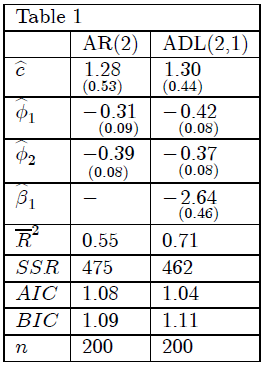
\includegraphics{tute12_1}}
	\end{figure}
	\vspace{-\baselineskip} \noindent which model do you prefer? Briefly explain.}

\noindent Since both models have the same dependent variable $y$, we can use the $\bar{R}^2$, $AIC$, and $BIC$ to choose a preferred model for $y$. We prefer the model with:
\begin{itemize}\vspace{-\baselineskip}
	\item A higher $\bar{R}^2$
	\item A lower $AIC$
	\item A lower $BIC$
\end{itemize}\vspace{-\baselineskip} \noindent Since the ADL(2,1) model has the higher $\bar{R}^2$ and lower $AIC$, \begin{align*}
	\bar{R}^2_{ARDL(2,2)} = 0.71 &> \bar{R}^2_{AR(2)} = 0.55 \\
	AIC_{ARDL(2,2)} = 1.04 &< AIC_{AR(2)} = 1.08
\end{align*} we prefer the ADL(2,1). We are further in favour of ADL(2,1) model of $y$ because $\hat{\beta}_1$ has a test statistics equal to $$\dfrac{-2.64}{0.46} = -5.74$$ which makes $x_{t-1}$ statistically significant in explain $y_t$ (at any reasonable level of significance).

\noindent However, it is not incorrect to prefer the AR(2) model because it is more parsimonious and has a lower BIC than the ADL(2,1) model.

\noindent There are no unique correct answer, but there are wrong answers.

\noindent Explain why it is incorrect to say: \vspace{-\baselineskip} \begin{center}
	\textit{My preferred model is ADL(2,1) because it has the smaller Sum of Squared Residuals (SSR)}
\end{center}\vspace{-\baselineskip}  \noindent Because the ADL(2,1) model has the same regressors as the AR(2) model plus 1 additional regressor so its SSR is necessarily smaller.

\noindent \textcolor{red}{(b) When the researcher estimated the model $$y_t = c + \beta_0D_t + \phi_1y_{t-1} + \phi_2y_{t-2} + \beta_1x_{t-1} + \beta_2(D_tx_{t-1}) + u_t$$ by OLS where, \begin{equation*}
	D_t = \begin{cases}
	1 & for\ t=1,2,\dots,100 \\
	0 & for\ t=101,102,\dots,200
	\end{cases}
\end{equation*} he obtain the results reported below (standard errors are reported in parenthesis): $$\hat{y}_t = \underset{(0.44)}{1.32} + \underset{(0.04)}{0.30}D_t - \underset{(0.07)}{0.39}y_{t-1} - \underset{(0.06)}{0.31}y_{t-2} + \underset{(0.41)}{2.15}x_{t-1} + \underset{(0.07)}{0.15}(D_tx_{t-1})$$ $$SSR = 450 \quad \bar{R}^2 = 0.69 \quad n=200$$}

\noindent \textcolor{red}{i. What is $$\hat{E}(y_t|y_{t-1}, y_{t-2}, x_{t-1})$$ for different values of $t$. Briefly explain.}

\noindent Since \begin{align*}
 y_t &= c + \beta_0D_t + \phi_1y_{t-1} + \phi_2y_{t-2} + \beta_1x_{t-1} + \beta_2(D_tx_{t-1}) + u_t \\
 &= {E}(y_t|y_{t-1}, y_{t-2}, x_{t-1}, D_t) + u_t 
\end{align*} \noindent that is, $${E}(y_t|y_{t-1}, y_{t-2}, x_{t-1}, D_t) = c + \beta_0D_t + \phi_1y_{t-1} + \phi_2y_{t-2} + \beta_1x_{t-1} + \beta_2(D_tx_{t-1})$$ so the estimated conditional expectation of $y_t$ is given by,
\begin{align*}
	\hat{E}(y_t|y_{t-1}, y_{t-2}, x_{t-1}, D_t) &= \hat{c} + \hat{\beta}_0D_t + \hat{\phi}_1y_{t-1} + \hat{\phi}_2y_{t-2} + \hat{\beta}_1x_{t-1} + \hat{\beta}_2(D_tx_{t-1}) \\
	&= 1.32 + 0.30D_t - 0.39y_{t-1} - 0.31y_{t-2} + 2.15x_{t-1} + 0.15(D_tx_{t-1})
\end{align*} It follows that 
$$\hat{E}(y_t|y_{t-1}, y_{t-2}, x_{t-1})$$ for different values of $t$ i.e.\vspace{-\baselineskip} \begin{itemize}
	\item $D_t = 1$ for $t=1,2,\dots,100$  
	\item $D_t = 0$ for $t=101,102,\dots,200$ 
\end{itemize} \vspace{-\baselineskip} is given by, 
\begin{equation*}
\hat{E}(y_t|y_{t-1}, y_{t-2}, x_{t-1}) = \begin{cases}
1.62 - 0.39y_{t-1} - 0.31y_{t-2} + 2.30x_{t-1} \quad for\ t=1,2,\dots,100 \\
1.32 - 0.39y_{t-1} - 0.31y_{t-2} + 2.15x_{t-1} \quad for\ t=101,102,\dots,200
\end{cases}
\end{equation*}

\noindent \textcolor{red}{ii. What is the estimated immediate and long run effect of a one unit increase in $x$ on $y$ before and after time $t=100$. Briefly explain.}

\noindent Since $x_t$ is not included in either equations, $x$ does not have an immediate effect on $y$ before or after time 100. 

\noindent The estimated long run effect on $y$ of a unit increase in $x$ $$= \dfrac{sum\ of\ estimated\ coefficients\ x_t\ and\ its\ lags}{1 - sum\ of\ estimated\ coefficients\ of\ lags\ of\ y_t}$$ $\therefore$ the estimated long run effect on $y$ of a unit increase in $x$ before and after time 100 \begin{align*}
	\dfrac{2.30}{1 - (-0.39 - 0.31)} & = 1.35 \quad for\ t=1,2,\dots,100 \\
	\dfrac{2.15}{1 - (-0.39 - 0.31)} & = 1.26 \quad for\ t=101,102,\dots,200
\end{align*}

\noindent \textcolor{red}{iii. Test the null \textbf{hypothesis} that there is no structural break in either the intercept or the coefficient attached to $x_{t-1}$ in the ADL(2,1) model. State the null and alternative hypothesis, the form of the asymptotic distribution of the test statistic under the null, the sample value and critical value of the test statistic and your conclusion.}

\noindent Structural break - change in the coefficient after some time period $$y_t = c + \beta_0D_t + \phi_1y_{t-1} + \phi_2y_{t-2} + \beta_1x_{t-1} + \beta_2(D_tx_{t-1}) + u_t$$
\vspace{-\baselineskip}
\begin{align*}
	H_0&: \beta_0 = \beta_2 = 0 \\
	H_1&: \beta_0\ and/or\ \beta_2 \neq 0
\end{align*} \vspace{-\baselineskip} $$F = \dfrac{(SSR_r - SSR_{ur})/2}{SSR_{ur}/(200-5-1)} \sim F_{2,200-5-1} \quad under\ H_0$$ 
\noindent The $SSR_{ur}$ is given in (b) and $SSR_{r}$ is given in the ADL(2,1) model in (a) Table 1,
$$SSR_{ur} = 450 \quad SSR_{r} = 462$$
$$F_{calc} = \dfrac{(462 - 450)/2}{450/194} = 2.59$$ $$F_{crit} \approx 3.07$$
\noindent Since $F_{calc} = 2.59 < F_{crit} \approx 3.07$ we fail to reject the null and conclude that there is insufficient evidence from our sample of a structural break in either the intercept or the coefficient of $x_{t-1}$. (Correct to say that sample size used to estimate the model is 198 $\therefore\ F_{2,198-5-1}$ because 2 observations were loss by including a variable lagged 2 periods as a regressor.)

\noindent \textcolor{red}{(c) Carefully describe the steps involved in performing a \textbf{Breusch-Godfrey test} for autocorrelation up to order 2 in the error term in the ADL(2,1) model $$y_t = c + \phi_1 y_{t-1} + \phi_2 y_{t-2} + \beta_1 x_{t-1} + u_t.$$ Make sure you specify the form and the distribution of the test statistic.}

\noindent We are testing for serial correlation in $u_t$ up to order 2, so we specify a model of $dlgdp$ with errors that follow an AR(2) process.
\begin{align*}
y_t &= c + \phi_1 y_{t-1} + \phi_2 y_{t-2} + \beta_1 x_{t-1} + u_t \\
u_t &= \rho_1u_{t-1} + \rho_2u_{t-2} + e_t
\end{align*} $$e_t \sim WN(0,\sigma^2)$$ $$(e_t \sim i.i.d(0,\sigma^2)\ also\ okay)$$
\begin{align*}
H_0&: \rho_1 = \rho_2 = 0 \\
H_1&: at\ least\ one\ of\ the\ above\ \rho \neq 0
\end{align*}
To perform the Breusch-Godfrey test for serial correlation in the errors of model $y_t$ up to order 2,
\begin{itemize}
	\item Estimate the model $$y_t = c + \phi_1 y_{t-1} + \phi_2 y_{t-2} + \beta_1 x_{t-1} + u_t$$
	\item Save the residuals from the above estimated model 
	\item Then estimate the following $auxiliary\ regression \dots$ $$\hat{u}_t = \alpha_0 + \alpha_1y_{t-1} + \alpha_2y_{t-2} + \alpha_3x_{t-1} + \rho_1\hat{u}_{t-1} + \rho_2\hat{u}_{t-2} + v_t$$
	\item The test statistic is $$BG = n_{aux} \times R^2_{aux} \overset{asy}{\sim} \chi^2_2 \quad under\ H_0$$ where $n_{aux}$ is the number of observations in the auxiliary regression
	\item  Calculate the test statistic $$BG_{calc}$$ and we reject the null of $$BG_{calc} > BG_{crit}$$ where $$BG_{crit} = \chi^2_{0.95,2} = 5.99$$. If we reject the null then there is evidence of serial correlation in the errors.
\end{itemize}













\end{document}
